\documentclass{beamer}


\usepackage[french,english]{babel}

\usepackage[T1]{fontenc}

\usepackage[utf8]{inputenc}


\usetheme{Warsaw}
\title{Résultats de l'heuristique}

\author{Clément Legrand}
\date{7 Juin 2018}

\begin{document}

\section{Exécution de l'heuristique}

\begin{frame}[plain]
\titlepage
\end{frame}

\begin{frame}{Exécution}
\begin{block}{Détail}
\begin{itemize}
\item Calcul SI avec CW, et amélioration avec LK;
\item Itérations en exécutant successivement EC, CE, LK.
\item On repart de la dernière solution globale toutes les $25$ itérations sans améliorations;
\item Si on trouve une amélioration, on met à jour la solution globale;
\item Toutes les $100$ itérations sans améliorations, on change de fonction de pénalisation.
\item On quitte la boucle au bout de $1500$ itérations successives sans améliorations;
\item A la fin on essaie de supprimer toutes les routes qui n'ont qu'un client.
\end{itemize}
\end{block}
\end{frame}

\section{Présentation résultats}

\subsection{Résultats}

\begin{frame}{Instance A-n37-k06}
Exécution de l'heuristique sur des instances de la littérature:
\begin{center}
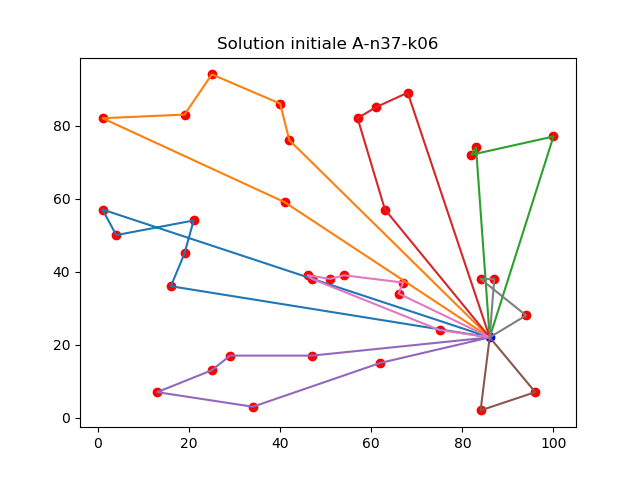
\includegraphics[scale=0.3]{initiale_A-n37-k06.png}
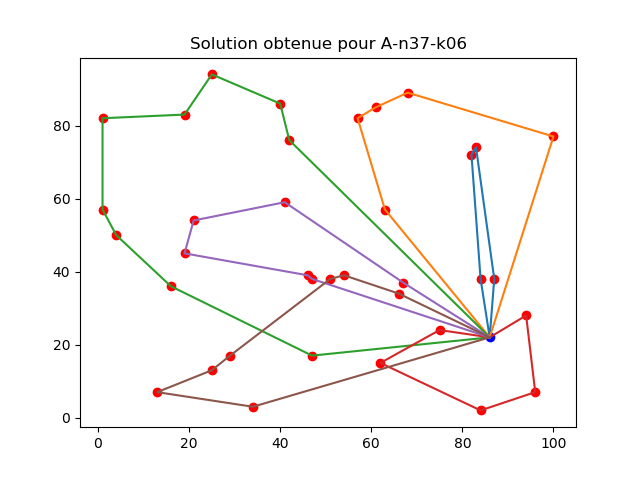
\includegraphics[scale=0.3]{solution_A-n37-k06.png}
\end{center}

\end{frame}

\begin{frame}{Comparaison}
Pour pouvoir comparer entre la solution optimale et la solution obtenue:
\begin{center}
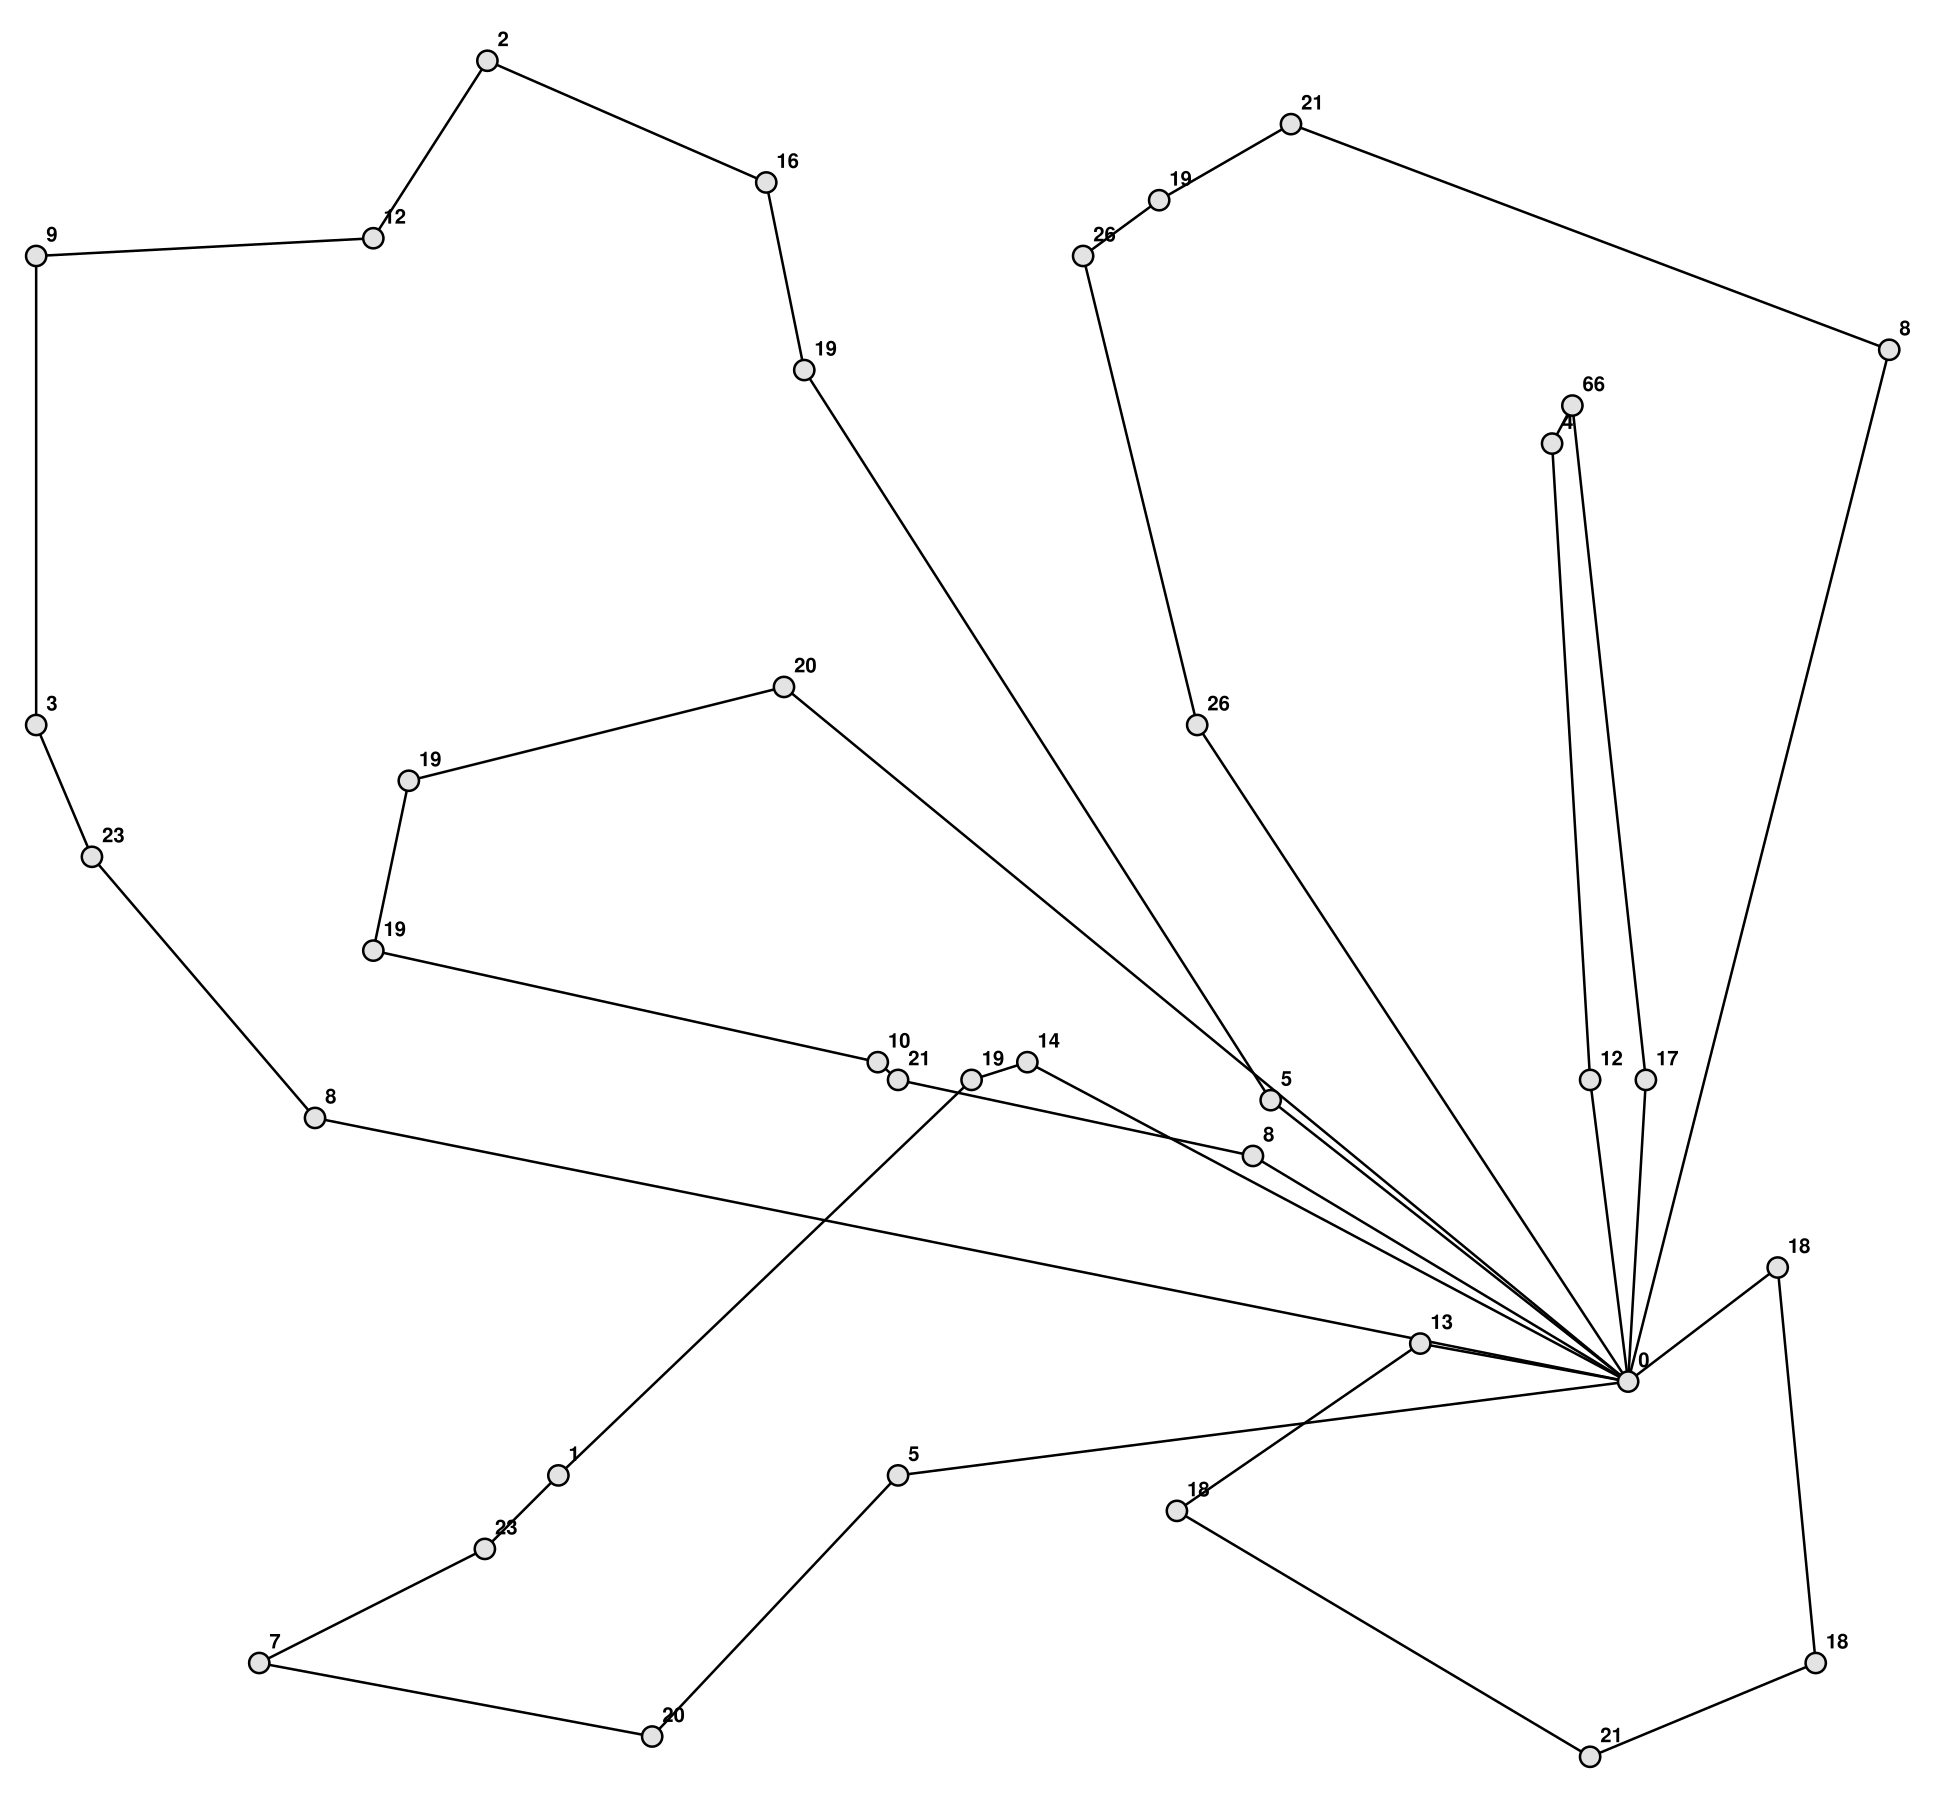
\includegraphics[scale=0.25]{A-n37-k6.png}
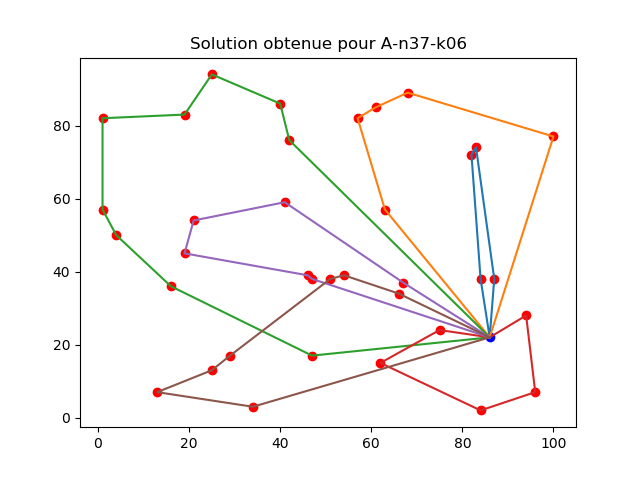
\includegraphics[scale=0.35]{solution_A-n37-k06.png}
\end{center}
Coût global de $949$ (à gauche), contre $952$ (à droite).
\end{frame}

\begin{frame}{Instance A-n39-k05}
Nouvelle instance choisie:
\begin{center}
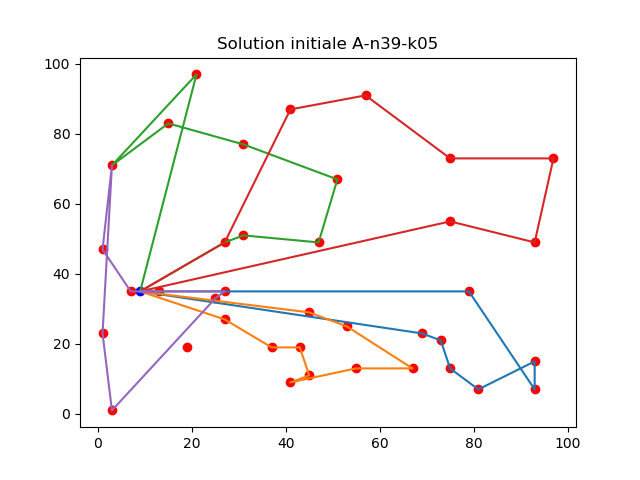
\includegraphics[scale=0.3]{initiale_A-n39-k05.png}
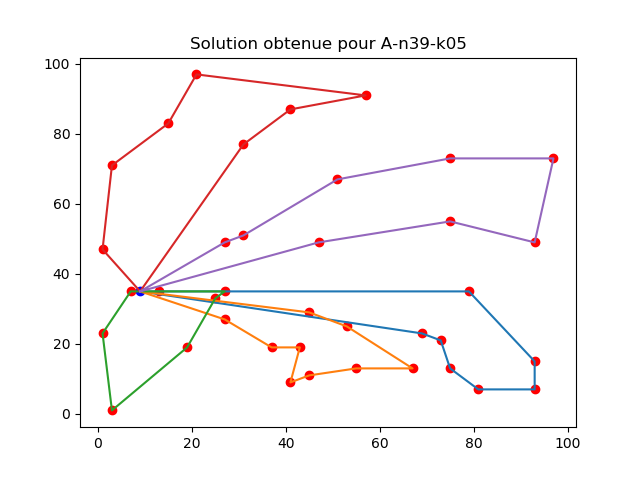
\includegraphics[scale=0.3]{solution_A-n39-k05.png}
\end{center}

\end{frame}

\begin{frame}{Comparaison}
Comparaison avec la solution optimale:
\begin{center}
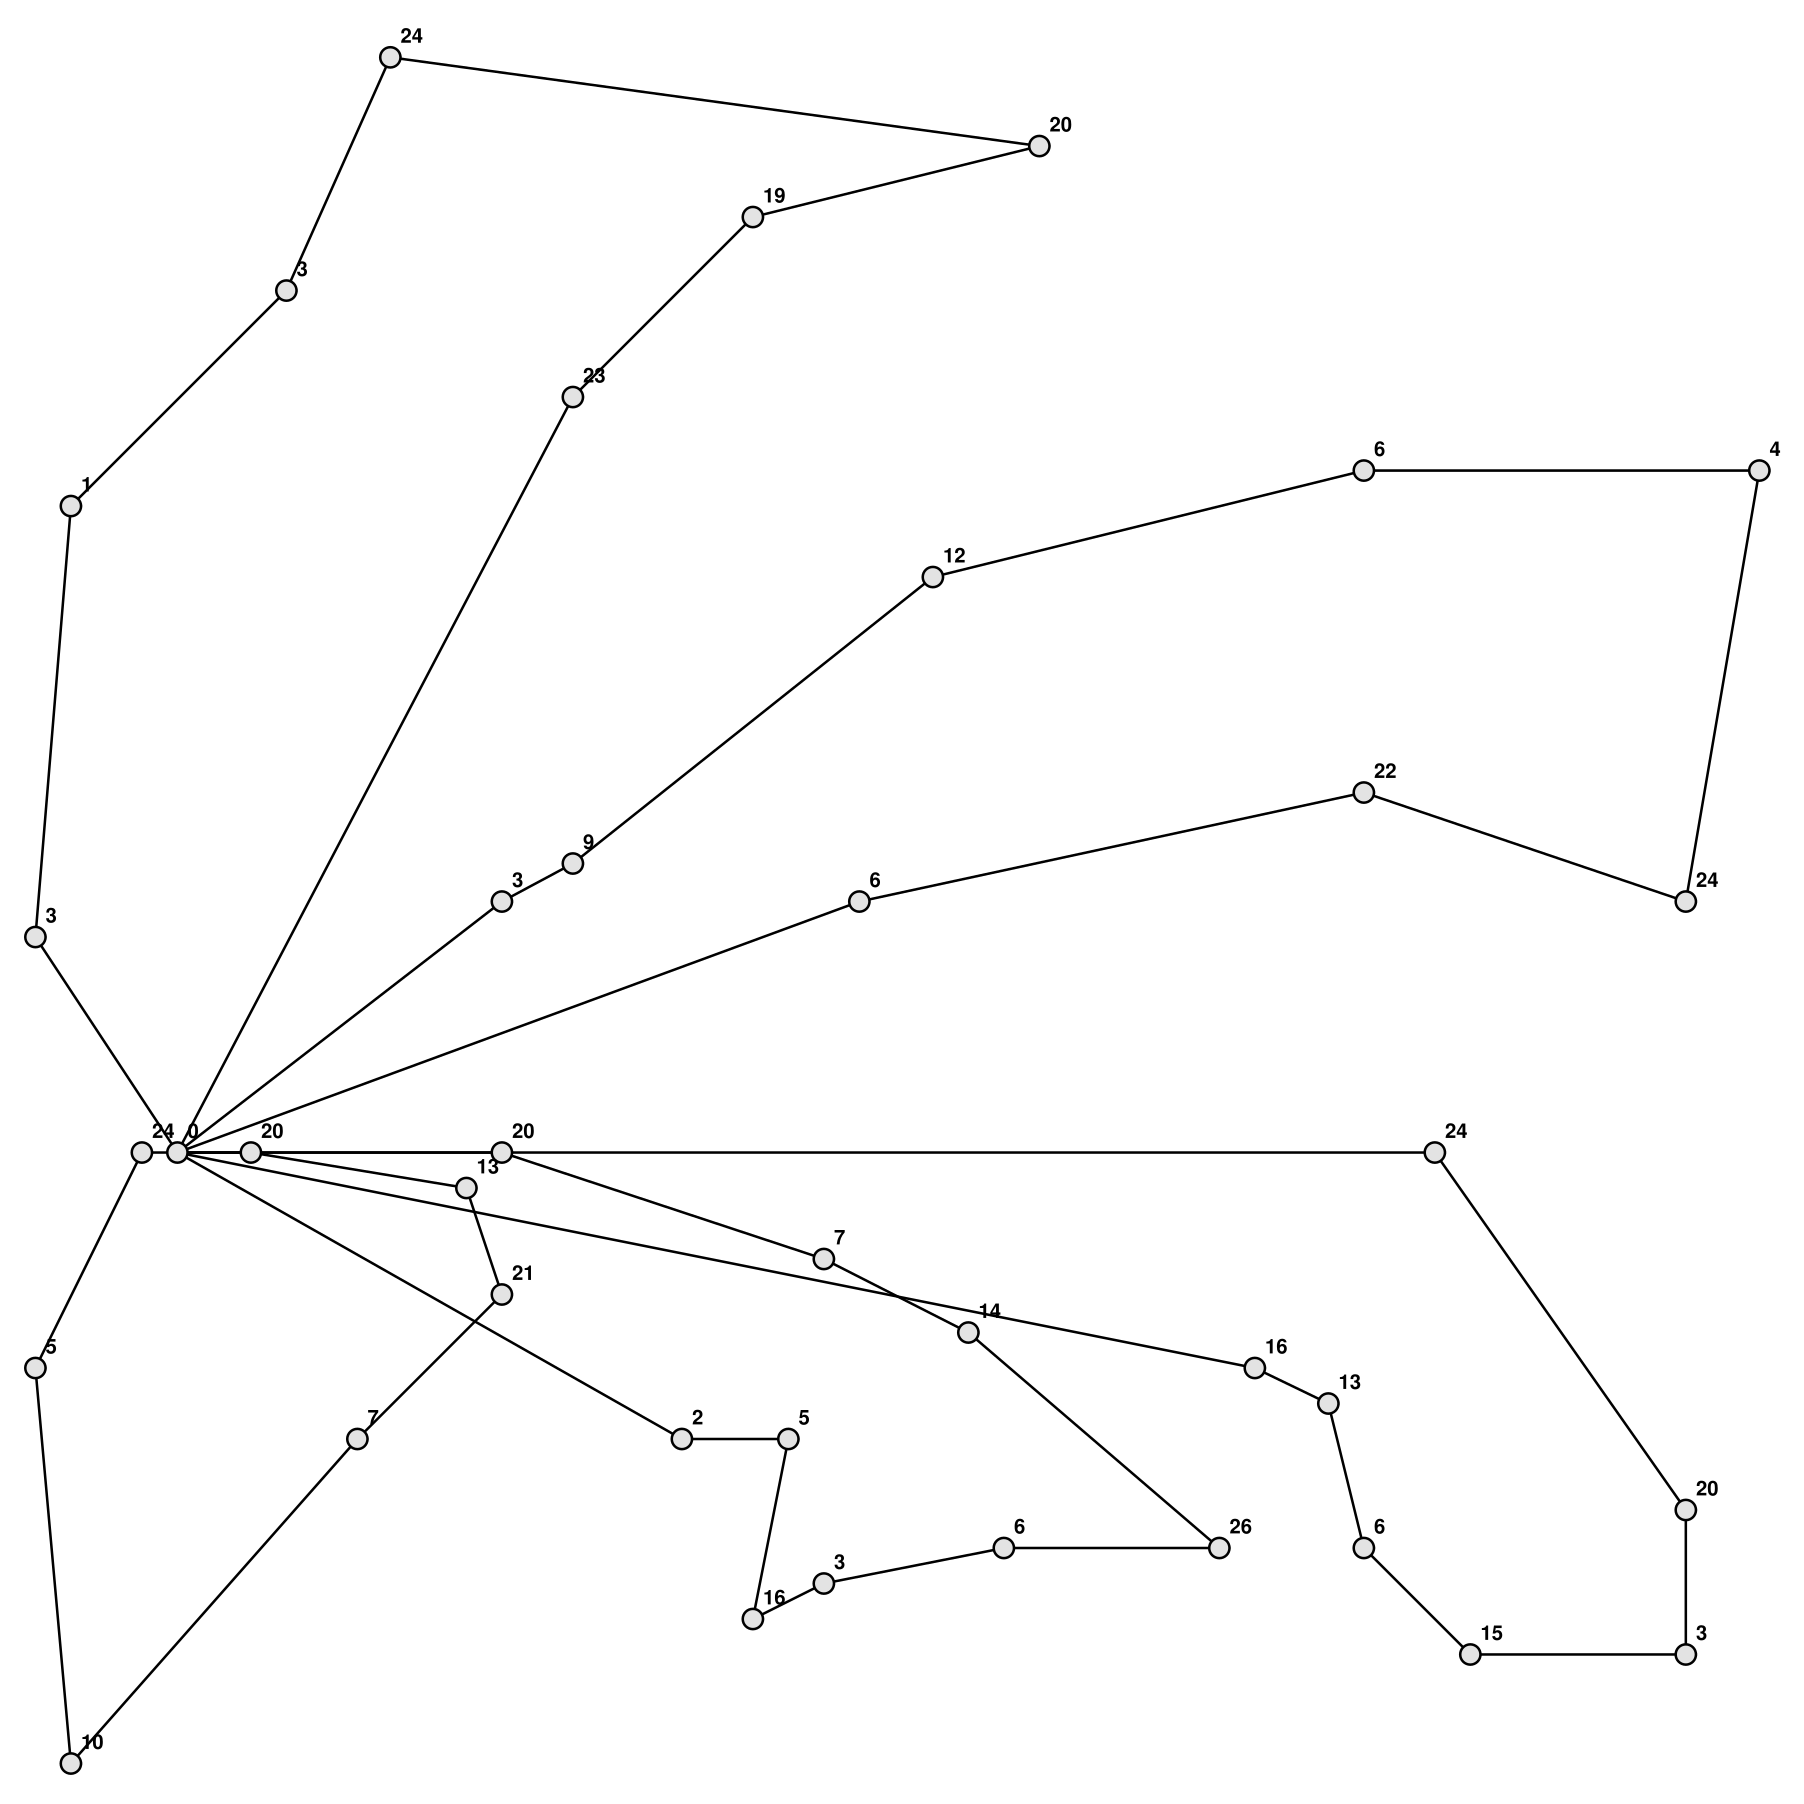
\includegraphics[scale=0.25]{A-n39-k5.png}
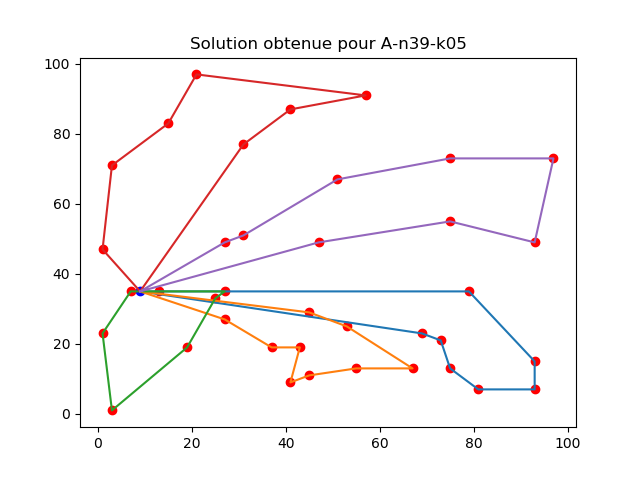
\includegraphics[scale=0.35]{solution_A-n39-k05.png}
\end{center}
Coût global de $822$ (à gauche), contre $831$ (à droite).
\end{frame}

\subsection{Analyse}

\begin{frame}{Paramètres utilisés}
Paramètres qui restent fixes dans l'heuristique:
\begin{block}{Valeurs choisies}
\begin{itemize}
\item Calcul des 30 pp-voisins;
\item Au plus 3 déplacements dans EC;
\item Arrêt au bout de $1500$ itérations sans améliorations.
\end{itemize}
\end{block}
Déterminées grâce à l'article et de manière empirique.
\end{frame}

\begin{frame}{Analyse}
Calcul du pourcentage d'erreur avec $1-\frac{c_{opt}}{c_{sol}}$
\begin{exampleblock}{Pourcentage d'erreur}
Sur $10$ instances, $0.8\%$ d'erreurs entre les solutions calculées et les solutions optimales. min = 0\% et max = 2.2\%. ($Q_1 = 0.34$, $ med = 0.69$, $Q_3 = 1.18$). 
\end{exampleblock}

\begin{alertblock}{Influence solution initiale}
Les solutions obtenues avec l'heuristique dépendent de la solution initiale: meilleures SI $\nRightarrow$ meilleures SG 
\end{alertblock}

\end{frame}

\begin{frame}{Exemples}
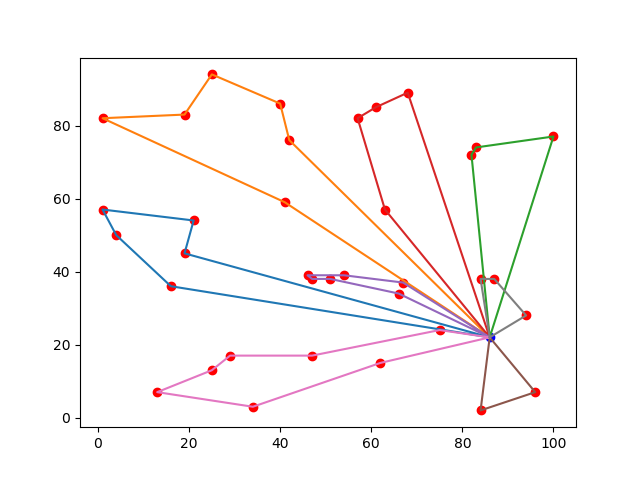
\includegraphics[scale=0.3]{bestInitiale_A-n37-k06.png}
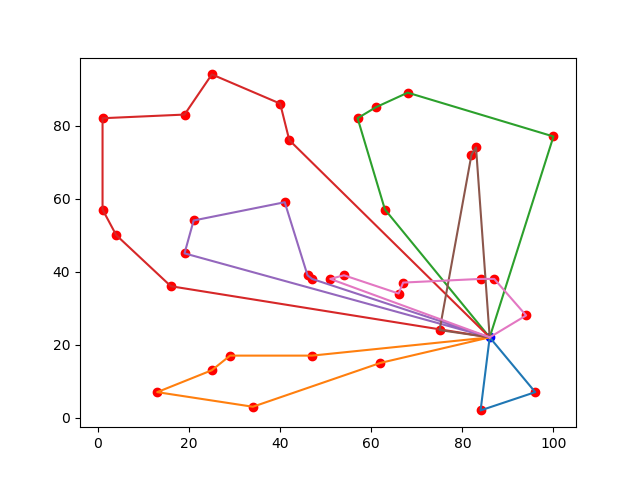
\includegraphics[scale=0.3]{badSolution_A-n37-k06.png}
Passage d'un coût de $1093$ (à gauche), à $1004$ (à droite).
\end{frame}

\begin{frame}{Exemples}
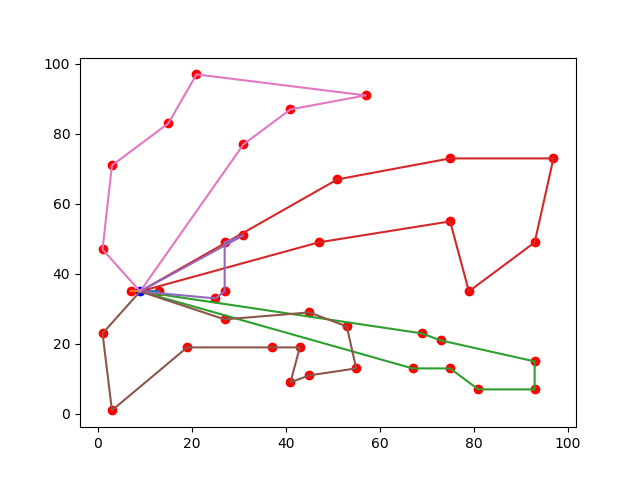
\includegraphics[scale=0.3]{bestInitiale_A-n39-k05.png}
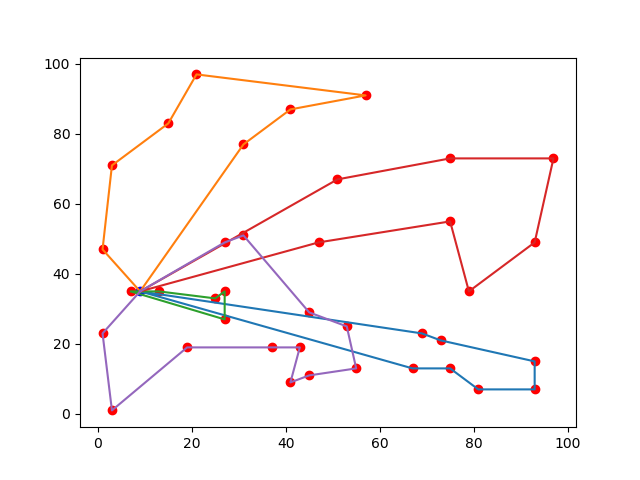
\includegraphics[scale=0.3]{badSolution_A-n39-k05.png}
Passage d'un coût de $1010$ (à gauche), à $837$ (à droite).
\end{frame}

\section{Arêtes communes}

\begin{frame}{Présentation}
Arêtes restées inchangées lors de l'algorithme:

\begin{center}
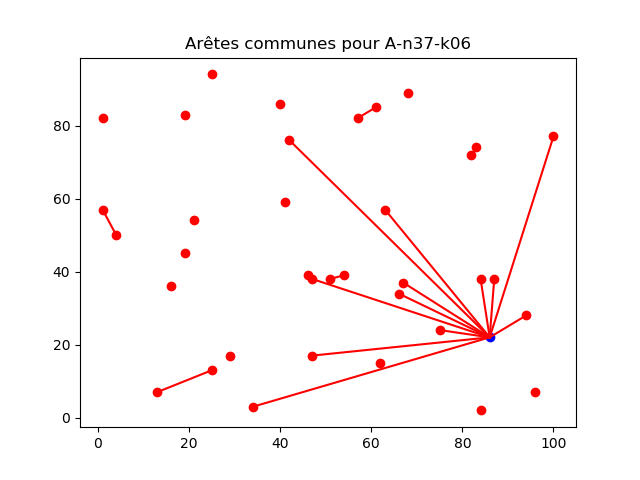
\includegraphics[scale=0.30]{commonEdges_A-n37-k06.png}
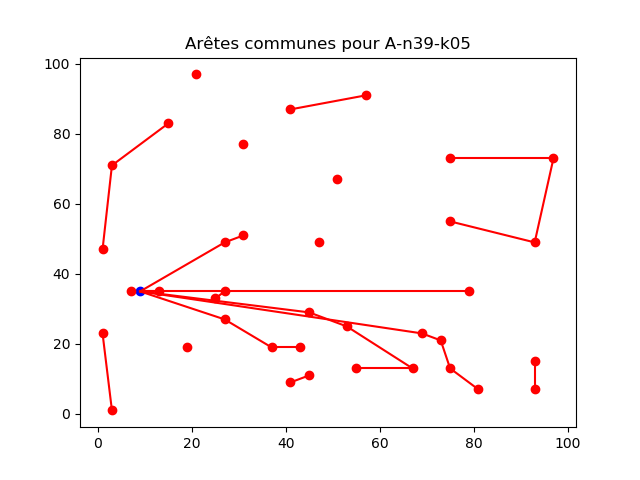
\includegraphics[scale=0.30]{commonEdges_A-n39-k05.png}
\end{center}

\end{frame}

\begin{frame}{Caractéristiques de ces arêtes}

\end{frame}
\end{document}